\chapter{Description of AMR-Based Detonation Solver in OpenFOAM}
\label{math}

\section{Overview}
OpenFOAM is a C++ toolbox that is a collection of various programs that is primarily used to solve computational fluid dynamics problems. Unlike many commercial CFD codes available, OpenFOAM does not use a GUI for problem setup and instead relies on the user to provide the toolbox a variety of text-based input files in which it interprets and uses for deriving a solution to a particular problem of interest. This is a blessing in disguise, as it allows for very clear control over what OpenFOAM does. Since the source is open, many additional tools and solvers have been developed for OpenFOAM, making it very flexible. The solvers tested during this research include:
\begin{itemize}
    \item \textbf{rhoReactingFoam}: a solver included with the OpenFOAM installation, in which the provided description calls it a ``[s]olver for combustion with chemical reactions using density-based thermodynamics package."
    \item \textbf{rhoCentralFoam}: a solver included with the OpenFOAM installation, in which the provided description calls it a ``Density-based compressible flow solver based on central-upwind schemes of Kurganov and Tadmor with support for mesh-motion and topology changes."
    \item \textbf{rhoReactingCentralFoam}: a solver developed by Caelan Lapointe at the University of Colorado Boulder, combining \verb|rhoReactingFoam| and \verb|rhoCentralFoam| together as well adaptive mesh refinement support. 
\end{itemize}

In addition to these solvers, several additional tools outside the standard OpenFOAM installation were utilized. This includes \verb|funkySetFields|, included with \verb|swak4Foam| \cite{swak4foam}. \verb|funkySetFields| is a tool much like the OpenFOAM-included \verb|setFields| utility, which allows the user to define set values of variables within certain regions of the computational domain (e.g. allows the user to set a cube within a domain to a certain temperature which is different than what is set globally). \verb|funkySetFields| extends this functionality, allowing for time and position-dependent defining of variables, such that an initial condition such as a temperature ramp, or randomization of temperature within the domain is possible. 

\section{Governing Equations}
In order to model detonations, the problem can be broken up into smaller pieces and solved with CFD. OpenFOAM is computational toolbox that will utilize the finite volume method (FVM) to solve the set of partial differential equations describing the fluid flow. In the FVM, the computational domain is broken into multiple smaller control volumes, known as cells. Each cell contains a set of thermo-fluid properties at the centroid. The differential equations are then integrated over this control volume in order to obtain a solution at each cell. The solution is interpolated between cell centroids to obtain a solution throughout the domain. 

The solution for the fluid problem explored in this thesis work is approximated through density, momentum, species, and energy equations. The solver used to approximate these equations in a discretized computational domain, \verb|rhoReactingCentralFoam|, utilizes the central-upwind schemes developed by Kurganov and Tadmor \cite{kurganov1}. The density equation solved by \verb|rhoReactingCentralFoam| is
\begin{equation}
\frac{\partial \rho}{\partial t} + \nabla \cdot \left(\rho \bm{u}\right) = 0\,,
\end{equation}
the momentum equation is
\begin{equation}
\frac{\partial \rho\bm{u}}{\partial t} + \nabla \cdot \left(\rho \bm{u}\otimes \bm{u}\right) + \nabla p = \bm{0}\,,
\end{equation}
the energy equation is
\begin{equation}
\frac{\partial \rho E}{\partial t} + \nabla \cdot \left[\left(\rho E + p\right)\bm{u}\right] = \dot{q}\,,
\end{equation}
and the species equation is
\begin{equation}
\frac{\partial \rho Y_i}{\partial t} + \nabla \cdot \left(\rho Y_i \bm{u}\right) = \dot{\omega}_i\,,
\end{equation}
where 
\begin{equation}
\dot{q} = \sum_{i = 1}^N \dot{\omega_i} \Delta h_{f,i}^0\,,
\end{equation}
is the heat flux, $\dot{\omega}_i$ is the species source reaction rate, $\rho$ is the density, $\bm{u}$ is the fluid velocity vector, $Y_i$ is the mass fraction of the $i$th species, $E$ is the total energy, $p$ is the pressure, and $\Delta h_{f,i}^0$ is the species formation enthalpy.

These equations \cite{kuo}, known as the reactive Euler equations, are solved using OpenFOAM's differential equation time step integrators. Different equation solvers can be selected for different quantities of interest. For quantities like velocity, internal energy, and species, the preconditioned biconjugate gradient stabilized method is used (\verb|PBiCGStab| in OpenFOAM). For solvers like this, preconditioners can be selected as well as solution tolerance and relative tolerance. Preconditioners are computational operations done on the solution matrix in order to help prepare them for numerical iterative solving such that less iterations are required. The system is closed when energy is expanded and an equation of state is added. Total energy \cite{kuo} can be written as 
\begin{equation}
E = h - \frac{p}{\rho} +\frac{1}{2} \left(\bm{u}\cdot\bm{u}\right)\,,
\end{equation}
where the total summed enthalpy is written \cite{kuo} as 
\begin{equation}
h = \sum_{i = 1}^Nh_{s,i}Y_i\,,
\end{equation}
and the species total enthalpy \cite{kuo} is given by 
\begin{equation}
h_{i} = \Delta h_{f,i}^0 + h_{s,i}\,,
\end{equation}
with the sensible enthalpy for the $i$th species expressed as
\begin{equation}
h_{s,i} = \int_{T_0}^T C_{p,i}\mathrm{d}T\,,
\end{equation}
Here $C_{p,i}$ is the specific heat for the $i$th species, $T$ is the temperature, and $T_0$ is an initial, or reference, temperature. The equation of state is expressed as 
\begin{equation}
p = \rho R T\,,
\end{equation}
where $R=R_u/W$, with $R_u$ the universal gas constant and $W$ is the mixture molecular weight. Transport coefficients were represented using the Sutherland model, given as \cite{ofug}:
\begin{equation}
\mu = \frac{A_s \sqrt{T_s}}{1 + \frac{T_s}{T}} \,,
\end{equation}
where $\mu$ is the dynamic viscosity, $A_s$ is the Sutherland coefficient, and $T_s$ is the Sutherland temperature. 

Since detonation modeling consists of both a fluids problem as well as chemical problem, chemical reactions must also be considered. Like a fire, a detonation requires a fuel and an oxidizer. Typically, detonations in experimental and computational modeling will utilize gaseous hydrogen or methane fuels mixed with air or pure oxygen oxidizers. For the computational modeling here, hydrogen-air was the primary respective fuel-oxidizer combination utilized for exploring detonation modeling. This was due to the highly reactive nature of hydrogen as well as previous computational and experimental modeling resources available. The reaction used \cite{kuo} for the hydrogen detonation modeling here is
\begin{center}
%\ch{Na2SO4 ->[ H2O ] Na+ + SO4^2-}
\ch{2 H2 + 2 (O2 + 3.76 N2) -> 2 H2O + 7.52 N2}
\end{center}
This is a stoichiometric reaction between diatomic hydrogen gas and air. When converted to mass fraction \(Y\) for OpenFOAM \cite{marcantoni}, it becomes Table \ref{tab:y}.

\begin{table}[t!]
\centering
\caption{Species mass fraction initial condition}
\label{tab:y}
\begin{tabular}{cc}
Specie & Mass Fraction \\ \hline
H\(_2\) & 0.02851 \\ 
H\(_2\)O & 0 \\
N\(_2\) & 0.745 \\ 
O\(_2\) & 0.226 \\ 
Total & 0.99951 \\ 
\end{tabular}
\end{table}

Other trace elements present in air are not modeled here, and this could be a topic of further study within the context of OpenFOAM detonation modeling with AMR. Additionally, a single-step reaction was modeled as opposed to several reactions together to model hydrogen-air detonations. While more steps are certainly more realistic, adding further reaction complexity was found to significantly increase computational expense. It was decided that gaining a better baseline understanding of how AMR could improve modeling efficiency in OpenFOAM was the focus here and thus further work on increasing the reaction complexity and accuracy was not performed. 

The chemical reaction rate can be modeled OpenFOAM with the Arrhenius equation \cite{christ} which takes the form
\begin{equation}
\dot{\omega}_i = AT^\beta \exp\left(\frac{E_a}{R T}\right)\,,
\end{equation}
where $A$ is the pre-exponential factor, $\beta$ is the temperature exponent, and $E_a$ is the activation energy. OpenFOAM requests \verb|A|, \verb|beta|, and \verb|Ta|. We can write \(Ta = \frac{Ea}{R }\). While in later sections the effect of \(A\) is explored on the solution, the values landed on for numerical simulation in this work are:
\begin{equation}
   A = 1.4 \times 10^{13} ~ \text{m}^3\text{mol}^{-1}s^{-1},
   \qquad 
   Ta = 12996 ~\text{K},
   \qquad
   \beta = 0\,.
\end{equation}
\noindent In addition, the specific gas constant used is \(R = 368.9\) J/Kg-K. It is seen in Chapter \ref{sec:a} that the values used are reasonably close to Chapman-Jouguet theory as well as other published values \cite{towery1}\cite{hashemi}. 

\section{Numerical Methods}
Within OpenFOAM, a user can choose how to numerically solve the stiff set of differential equations that model reacting flows. Thermodynamic variables such as specific heat can be selected to be temperature-dependent using polynomial approximations such as those given by the JANAF tables, such that \(C_{p,i} = C_{p,i}(T)\). No significant increase in complexity of the solution was noticed, so JANAF settings were used for temperature-dependent thermodynamics. The energy equation solution variable can also be selected, such that either sensible enthalpy or sensible internal energy is solved, and we selected sensible internal energy for modeling detonations with \verb|rhoReactingCentralFoam|, since less numerical error was noticed in the solution, as compared to solutions using the sensible enthalpy. The numerical solution of the Euler equations in OpenFOAM occurs with several different settings. Different numerical schemes can be applied separately to variables of interest, and can be seen in Table \ref{tab:numschemes}. 

\begin{table}[t!]
\centering
\caption{OpenFOAM finite volume numerical schemes applied during solving}
\label{tab:numschemes}
\begin{tabular}{ccc}
Term & OpenFOAM Variable & Numerical Scheme \\ \hline 
Flux Scheme & \verb|fluxScheme| & Kurganov \\ 
Time Scheme & \verb|ddtSchemes| & Euler \\
Gradient Schemes & \verb|gradSchemes| & Gauss linear \\ 
Divergence Schemes & \verb|divSchemes| & none by default \\ 
& \verb|div(tauMC)| & linear \\ 
& \verb|div(phi,|specie\verb|)| & van Leer \\ 
Laplacian Schemes & \verb|laplacianSchemes| & Gauss linear uncorrected \\ 
Interpolation Schemes & \verb|interpolationSchemes| & default linear \\
& \verb|reconstruct(rho)| & Minmod \\ 
& \verb|reconstruct(U)| & MinmodV \\ 
& \verb|reconstruct(T)| & Minmod \\ 
& \verb|reconstruct(Yi)| & Minmod \\ 
Surface Normal Gradient Schemes & \verb|snGradSchemes| & uncorrected \\
\end{tabular}
\end{table}

In Table \ref{tab:numschemes}, Gauss linear specifies two things \cite{ofug}. The ``Gauss'' portion specifies that OpenFOAM should use a standard finite volume Gaussian integration with interpolation of values of interest between face centers and cell centers. The ``linear'' portion tells OpenFOAM that piecewise linear interpolation should be used for the interpolation. It should be noted that the ``uncorrected'' term is a flag that tells OpenFOAM that the orthogonal component of a flow variable with respect to a cell face should not undergo a non-orthogonal correction, since structured grids are used in this research. ``Corrected'' is more useful for engineering geometries where the mesh faces are not always aligned with a Cartesian coordinate system. 

The next important scheme is the van Leer \cite{vanleer} flux limiting scheme that limits the solution gradient near regions such as shocks. Cell interpolation with this method is piecewise linear, but the slopes are limited. This scheme requires use of the linear Gudunov scheme that assumes a discontinuous solution on ever finite volume cell face. Like the van Leer scheme, Minmod is a slope limiter, but uses a different set of criteria for the limiting. Time integration is performed using the Euler scheme, which is a transient and first-order implicit scheme. This scheme relies on knowledge of the derivative and therefore both the current and subsequent solution in order to give an approximation of the solution at the next time step. By knowing the slope of the solution, we can guess the solution at the next time step by tracing out where it should be by this rate of change. The last numerical scheme used is the Kurganov scheme \cite{kurganov1}, a central difference scheme by Kurganov and Tadmor that is second order and high resolution. 

Once the numerical schemes are defined, the system of equations needs to be solved. The mass, momentum, energy, and species equations are combined together in matrix linear form to be solved (\(\bm{Ax} = \bm{b}\)). OpenFOAM allows the user to alter the solver settings for each solution variable\cite{ofug}. The velocity, internal energy, and species mass fraction utilize the PBiCGStab solver mentioned earlier. This is an iterative linear solver that uses a preconditioner to help accelerate convergence of the solution.  Computationally, there are two matrix-vector multiplications, six parallel reductions, and a twice-applied preconditioning step that occurs every time step. Upon startup there is an initial matrix-vector multiplication and a single parallel reduction. The preconditioner used for enthalpy and species is known as DILU, or Diagonal-based Incomplete LU. This preconditioner performs an incomplete LU factorization of the solution matrix and reduces the solver sensitivity to errors or changes in input. The preconditioner for velocity is DIC, or Diagonal-based Incomplete Cholesky. This preconditioner performs an incomplete Cholesky factorization of the solution matrix to precondition the solution matrix. Density is solved using the \verb|diagonal| solver, a simple solve by a solution matrix inversion. Parameters used for numerical solving can be seen in Table \ref{tab:numerics}. 

\begin{table}[t!]
\centering
\caption{Finite volume numerical solvers and preconditioners used for solution variables}
\label{tab:numerics}
\begin{tabular}{cccc}
Variable & Solver & Parameter & Value \\ \hline 
\verb|e|, \verb|Yi| & \verb|PBiCGStab| & Preconditioner & \verb|DILU| \\ 
& & Tolerance & \verb|1e-17| \\ 
& & Relative tolerance & 0 \\
\verb|U| & \verb|PBiCGStab| & Preconditioner & \verb|DIC| \\ 
& & Tolerance & \verb|1e-15| \\ 
& & Relative tolerance & 0 \\
\verb|rho| & \verb|diagonal| & & \\
\end{tabular}
\end{table}

The chemistry uses a separate solver than the rest of the reacting flow solution variables. The settings for the chemistry solver are found in \verb|constant/chemistryProperties|. The directory structure of OpenFOAM is discussed in greater detail in the next section. The chemistry is solved before the flow variables, with a separate initial time step. For detonation modeling presented here, the chemistry ordinary differential equation (ODE) is solved using the Runge-Kutta-Fehlberg method \cite{rkf}, known to OpenFOAM as RKF45. 

Together, the numerical schemes, numerical solvers, and chemistry solver combine to solve the reactive Euler equations as \verb|rhoReactingCentralFoam| within OpenFOAM. These solution techniques can then be applied to flow problems such as detonations. 

\section{Setup and Structure}
In order to simulate a fluids or combustion problem in OpenFOAM, the directory structure in which the simulation is to be run needs to be correct. Each OpenFOAM simulation contains a directory \verb|0/| which holds initial conditions for the domain as well as boundary conditions \cite{ofug}. Inside this directory are files named like the quantities they represent, such as \verb|p|, \verb|T|, and \verb|U|. \verb|funkySetFields| edits these files to apply the special initial conditions. As the simulation progresses, more folders representing timesteps will appear with data saved for that timestep. The folder name will represent the specific timestep exactly. 

The next important directory is \verb|constant/|. This directory holds physical quantities as well as mesh information once it is formed. For reacting flows, some files of interest within this folder may be:

\begin{itemize}
    \item \textbf{chemistryProperties}: a file that contains definitions for which chemistry solver is used as well as tolerances.
    \item \textbf{combustionProperties}: contains the combustion model (laminar, or turbulence model) definition.
    \item \textbf{dynamicMeshDict}: defines adaptive mesh refinement options. One can define which variable is tracked during adaptive meshing as well as how often and refined the meshing is. 
    \item \textbf{reactions}: contains all the reactions that occur during the simulation. The active species are defined here as well as the rate model (such as Arrhenius). 
    \item \textbf{thermo.compressibleGas}: included are the thermodynamic properties such as temperature-dependent specific heat coefficients and molecular weights of the species that are included within the chemistry models.
    \item \textbf{thermophysicalProperties}: defines things such as the equation of state, inert species, locations of \verb|reactions| and \verb|thermo.compressibleGas|, if the mixture is reacting, if the thermodynamic properties are temperature-dependent, and how the energy equation is defined (e.g. one can have the model focused on sensible enthalpy or sensible internal energy).
    \item \textbf{turbulenceProperties}: defines turbulence modeling for the flow in general. 
\end{itemize}

The last necessary directory is \verb|system/|. This directory contains files that will define some generic solver tolerances as well mesh setup and simulation setup. Specifically, it could contain:

\begin{itemize}
    \item \textbf{blockMeshDict}: defines the mesh. A user will input dimensions and how the hex mesh will be partitioned. This could also be placed within \verb|constant/polyMesh/|. 
    \item \textbf{controlDict}: the overarching control file for OpenFOAM. This contains start and end times, time increments, write-to-file frequency, save file compression and format, and adaptive time stepping parameters such as maximum Courant number. Other options such as functions for residual tracking and libraries for functions like \verb|funkySetFields| can be placed here. 
    \item \textbf{decomposeParDict}: defines parallel processing domain decomposition for MPI. The number of processors as well as where domain splits should occur or algorithm definitions for automatic domain decomposition are set here. 
    \item \textbf{setFieldsDict}/\textbf{funkySetFieldsDict}: defines custom field setting, as discussed earlier. Blocks of pressure or temperature ramps are defined here. 
    \item \textbf{fvSchemes}: finite volume methods are defined here, such as Gauss linear or van Leer MUSCL schemes. It is broken into derivative, gradient, divergence, laplacian, and more sections. 
    \item \textbf{fvSolution}: defines the specific differential equation solvers as well as their tolerances. This can also contain smoothers and other solver-specific settings. 
    \item any files that define sampling for post processing, such as line plots through a region in the domain.  
\end{itemize}

Together, these directories comprise the OpenFOAM directory structure. A user then will run the solver of interest within the directory containing these subdirectories, and the solver will look within these subdirectories for the files just discussed and apply them to the solution process. Pre-processing and post-processing steps are also run from this directory, such as creating the mesh from \verb|blockMesh|, placing special initial conditions with \verb|funkySetFields|, or obtaining results at a timestep with a line plot with \verb|postProcess|. Results can also be viewed graphically with \verb|paraview| or \verb|paraFoam|. 

At this stage, some modeling notation should be introduced to simplify some things. Initial and static grid resolutions will take the form ``Nx-Ny-Nz'' with N representing the number of evenly-spaced cells that will fill the dimension, and x/y/z representing the dimension. A 500-40-3 grid represents 500 cell divisions in x, 40 divisions in y, and 3 divisions in z. This notation will be used later to quickly distinguish between resolutions and dimensionality of a mesh. Since OpenFOAM does not strictly have a one-dimensional or two-dimensional operating mode, three dimensions must always be realized. This is not a problem however, as a single cell can be used to represent a flattened dimension, with special boundary conditions for the faces that are in the ``dimensionless'' plane. For example, a two-dimensional geometry would be represented with a 500-40-1 mesh, and a one-dimensional geometry with a 500-1-1 mesh. 

\begin{figure}[t!]
\centering
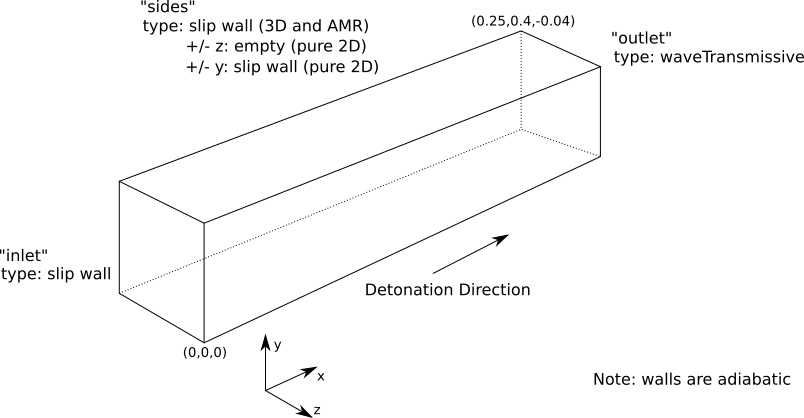
\includegraphics[width=\linewidth]{./figs/domainBC.png}
\caption{Geometry and domain setup with boundary conditions}
\label{fig:domainBC}
\end{figure}%

\section{Domain Setup}
The geometry used for this research is seen in Figure \ref{fig:domainBC}. The so-called ``inlet'' (even though fluid is not actively moving through this face) is the region where the detonation is initiated. The inlet is a solid adiabatic wall with velocity slip conditions such that the fluid can slide across it without effects from viscosity. This was chosen such that just the detonation itself can be studied in a pure form. Other walls are like this, such as the walls that make up the sides. It should be noted that the sides located in the x-y planes (``front and back'') change their type depending on the simulation. Since OpenFOAM does not have a two-dimensional mesh mode, for static mesh two-dimensional simulations these faces are set as a special ``empty'' patch type in order to tell OpenFOAM that it is a two-dimensional simulation taking place. For three-dimensional simulations the front and back faces are identical to the x-z ``top and bottom'' planes, which like the inlet are velocity-slip adiabatic walls. Two-dimensional AMR runs also use the three-dimensional wall setup here as the oct-tree cell splitting algorithm for mesh refinement is inherently three-dimensional even if we are simulating a two-dimensional domain. Due to this, two-dimensional simulations are actually pseudo-two-dimensional. 

The exit plane of the domain utilizes a ``waveTransmissive'' boundary condition. This is a special boundary condition that allows for waves such as shockwaves to not reflect at the boundary while expelling gases. A traditional OpenFOAM pressure outlet was seen to reflect the shockwave coupled with the detonation wave. 

The initial conditions for the domain are set at 300 K and 1 atm. An ignition region is initialized at a higher pressure and temperature at the start of the detonation tube and is discussed further in Section \ref{sec:ignition}.


%%%%%%%%%%%%%%%%%%%%%%%%%%%%%%%%%%%%%%%%%%%%%%%%%%%%%%%%%%%%
%%%%%%%%%%%%%%%%%%%%%%%%%%%%%%%%%%%%%%%%%%%%%%%%%%%%%%%%%%%%
%%%%%%%%%%%%%%%%%%%%%%%%%%%%%%%%%%%%%%%%%%%%%%%%%%%%%%%%%%%%


\section{Parallel Computing}
Included with the standard installation of OpenFOAM are solvers that are capable being scaled to make use of multiple processors \cite{ofug}. Solvers like \verb|rhoReactingCentralFoam| include this functionality. OpenFOAM's parallel processing is done through MPI, where several instances of a solver are run simultaneously and MPI passes information between the solvers. Each solver running in parallel computes on a different portion of the domain. 

In order to be able to run a solver in parallel, the domain must be decomposed into smaller pieces first. This is done with the \verb|decomposePar| utility, which takes user input from the \verb|decomposeParDict| file. Within this file, a user dictates how many times the domain is broken up, and how or where the domain is broken up. Several different decomposition methods can be utilized:
\begin{itemize}
\item \textbf{simple}: this is the most common method used for decomposition. The domain is split into chunks based on direction, and the user specifies how many splits there should be in each direction. 
\item \textbf{hierarchical}: similar to the \verb|simple| method, but instead an ordering to the domain splitting is used
\item \textbf{scotch}: this method does not require geometric input from the user but rather it attempts to minimize boundaries between processors. Processor weighting can be set. 
\item \textbf{manual}: cells are manually allocated to each processor here. 
\end{itemize}
In the researched performed here, the \verb|simple| method for domain decomposition was utilized due to the simplicity. Since detonations have small regions of high pressure, temperature, and velocity, some care must be done with respect to how the domain is decomposed, especially when considering AMR. If one were to decompose the domain into several pieces along the length of the tube, some processors would be working harder than other processors as the detonation passes into their respective domain chunks. We load balance the processors by not splitting the domain along the length of the detonation tube, and instead across it. This is shown in Figure \ref{fig:decomp}. 

\begin{figure}[p]
    \centering
    \begin{subfigure}[]{0.7\textwidth}
        \centering
        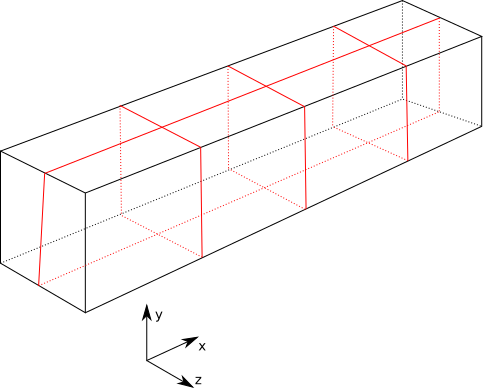
\includegraphics[width=\textwidth]{./figs/parallel_short.png}
        \caption{Domain decomposed into typical chunks, bad for detonation and AMR load balancing}
        \label{sfig:shortdecomp}
    \end{subfigure}

    \begin{subfigure}[]{0.7\textwidth}
        \centering
        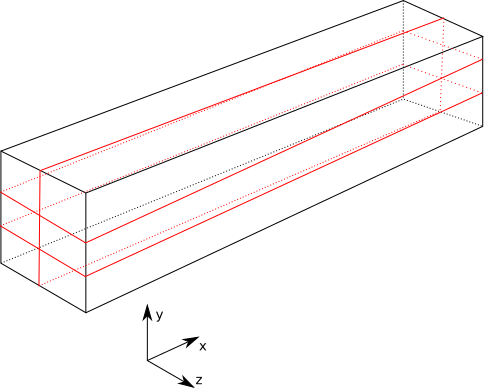
\includegraphics[width=\textwidth]{./figs/parallel_long.png}
        \caption{Domain decomposed into long chunks, better for detonation and AMR load balancing}
        \label{sfig:longdecomp}
    \end{subfigure}
    \caption{Example domain decomposition techniques for parallel computing}
    \label{fig:decomp}
\end{figure}%

Using long slivers seen in Figure \ref{sfig:longdecomp} instead of a typical aspect ratio consistent decomposition in Figure \ref{sfig:shortdecomp} allows for every processor to always have a small portion of the detonation in its domain. Otherwise, some processors would be waiting on other processors that have the detonation in them or heavy mesh refinement regions from the AMR routines.


%%%%%%%%%%%%%%%%%%%%%%%%%%%%%%%%%%%%%%%%%%%%%%%%%%%%%%%%%%%%
%%%%%%%%%%%%%%%%%%%%%%%%%%%%%%%%%%%%%%%%%%%%%%%%%%%%%%%%%%%%
%%%%%%%%%%%%%%%%%%%%%%%%%%%%%%%%%%%%%%%%%%%%%%%%%%%%%%%%%%%%


\section{Adaptive Mesh Refinement}

Adaptive mesh refinement is the process of refining or unrefining the computational mesh based on a tracked parameter of interest at a specific point in time. In OpenFOAM, AMR is available with several standard solvers such as \verb|interFoam|, and has been implemented into \verb|rhoReactingCentralFoam| by Caelan Lapoint. The AMR in this solver functions by looking within a mesh cell at a quantity of interest at a specific time interval, and deciding based on the value of that quantity of interest whether or not to refine the mesh in that cell. If the quantity is within the refinement bounds set by the user, the AMR routine will split the cell with an octree splitting method as shown in Figure \ref{fig:octree}. Additionally, the AMR can unrefine the mesh if the quantity of interest is outside the refinement bounds set by the user. The user settings are located within \verb|constant/dynamicMeshDict|, and several options exist for the user to tweak. Some of the most important ones include:
\begin{itemize}
\item \verb|dynamicFvMesh|: allows for the user to turn on and off the dynamic mesh refinement. 
\item \verb|refineInterval|: how often to do mesh refinement in terms of time step iteration. For example, a value of 2 here would mean that the AMR would look to refine or unrefine every other time step. 
\item \verb|field|: the variable of interest to track and refine based off of. If set as \verb|T|, AMR would check the temperature field values.  
\item \verb|lowerRefineLevel|: the lower bound for the AMR \verb|field| value tracking to refine upon. If the solution is higher than this bound during a \verb|refineInterval|, the cell will be refined. If the value is lower, it will not refine. 
\item \verb|upperRefineLevel|: the upper bound for the AMR \verb|field| value tracking to refine upon. If the solution is lower than this during a \verb|refineInterval|, the cell will be refined. If the value is higher, it will not refine. 
\item \verb|unrefineLevel|: the value of \verb|field| that will trigger unrefinement. If the value is less than this quantity, the AMR will unrefine cells. 
\item \verb|nBufferLayers|: how additional layers of cells will be refined around the cell that triggered a refinement. 
\item \verb|maxRefinement|: how many additional times cells can be refined within an iteration. 
\item \verb|maxCells|: the maximum number of cells in the computational domain that can be reached before adaptive mesh refinement is no longer performed. Note that this is not strictly followed but rather an estimate provided to the solver, since the octree splitting can potentially increase number of cells beyond this value at a specific iteration.
\end{itemize}
An exploration on how different selections in these parameters affects solution quality was performed in this research. Results will be shown in later chapter sections. An important aspect to note when utilizing \verb|rhoReactingCentralFoam|'s AMR is that the routine is inherently three-dimensional, due to the octree splitting method in Figure \ref{fig:octree}. 
\begin{figure}[b]
\centering
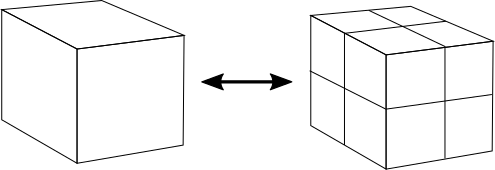
\includegraphics[width=0.6\textwidth]{./figs/amr_example.png}
\caption{Adaptive mesh refinement octree splitting method}
\label{fig:octree}
\end{figure}%
\noindent Due to this, one-dimensional simulations become pseudo one-dimensional, and two-dimensional simulations become pseudo two-dimensional, since cells will be added in all dimensions when refinement occurs. For detonation modeling in areas like detonation tubes, PDEs, and RDEs, this is acceptable as the velocity in other dimensions tends to be very small in comparison to the velocity in the detonation direction. 

Within \verb|dynamicMeshDict|, two main parameters can be used to guide the adaptive mesh refinement regionally to the target static mesh resolution. \verb|maxCells| stops the adaptive meshing from splitting and refining cells further once a \verb|maxCells| number of cells is reached in total throughout the domain. \verb|maxRefinement| tells the adaptive meshing routines how many further times per iteration it can split and refine cells, allowing for very fine cell resolution in small regions. The necessary number of refinement levels in a detonation simulation to reach target static cell resolution can be described with 
\begin{equation}
\verb|maxRefinement| \geq \log_2\left(\frac{N_{\text{static target}}}{N_{\text{AMR base}}}\right)
\end{equation}
where \(N_{\text{static target}}\) is the static mesh target resolution and \(N_{\text{AMR base}}\) is the unrefined base mesh resolution provided to the AMR simulation. For example, if our target static mesh had square cells and 5000 cells in length and the mesh we would like to use AMR with has 250 cells in length, this means that we need to use \(\verb|maxRefinement|\geq 5\) in order to reach the static mesh resolution. This does not guarantee that the simulation will be exactly as accurate as the static mesh resolution however, as other parameters such as the number of buffer cells, maximum number of cells, and more importantly the tracked field for refinement all change how the mesh will be refined. Note that the progression from refined cell to cell is also fairly smooth, such that a single octree touches each other. If a region needs to have lots of refinement, one must take this into account and provide the appropriate buffer layers with \verb|nBufferLayers| to allow the AMR to smoothly transition the mesh in time for the sensitive region to have an appropriate refinement level. The next parameter for mesh control discussed is \verb|maxCells|. 
%An approximation for the number of maximum cells in an AMR run can be described as the number of cells in the base AMR resolution plus the number of cells in the static region of interest. This will give extra cells for overlap and transition regions if one decides to use more buffer layers. Written, this is 
%\begin{equation}
%\verb|maxCells| \geq (N_xN_yN_z)_{\text{AMR base}} + 
%\end{equation}
The maximum number of cells can be estimated by considering the region where static mesh refinement needs to be active. By adding the number of cells in this region in the refined static mesh resolution to that of the base AMR resolution, an estimate for \verb|maxCells| can be determined. Note that if more buffer layers are utilized, \verb|maxCells| needs to be increased. 

In Figure \ref{fig:examr}, an example AMR detonation simulation is shown. The black boxes are the cell edges, and the adaptive meshing around the detonation wave can be clearly seen. 

\begin{sidewaysfigure}
\centering
\includegraphics[width=\textwidth]{./figs/amr_cells.png}
\caption{Three-level adaptive mesh refinement over a pressure field surface contour, with the detonation wave traveling from the -x wall to +x exit}
\label{fig:examr}
\end{sidewaysfigure}




%%%%%%%%%%%%%%%%%%%%%%%%%%%%%%%%%%%%%%%%%%%%%%%%%%%%%%%%%%%%
%%%%%%%%%%%%%%%%%%%%%%%%%%%%%%%%%%%%%%%%%%%%%%%%%%%%%%%%%%%%
%%%%%%%%%%%%%%%%%%%%%%%%%%%%%%%%%%%%%%%%%%%%%%%%%%%%%%%%%%%%


\section{Initial Meshing}
While the primary topic of interest in this work is adaptive meshing, a primary static mesh is required in order for the adaptive mesh refinement routines within OpenFOAM to refine from. Structured meshes are utilized, with hexahedrons making up the mesh. Meshes used for static mesh and initial AMR simulations can be seen in Figure \ref{fig:meshcompare}. The meshes displayed utilize 125 partitions along detonation ``tube'' and 20 partitions in width, depending on two or three dimensionality in order to be visible for the reader. Real meshes used in simulation are much more fine in order to capture the thin detonation and shock region. Meshes used in this research were created with the OpenFOAM utility \verb|blockMesh|, which generates structured hex meshes based on use input of ``blocks'' which define rectangular prisms that \verb|blockMesh| then uses to form faces and patches for boundary conditions as well as to partition into the mesh. 

\begin{figure}[]
    \centering
    \begin{subfigure}[]{\textwidth}
        \centering
        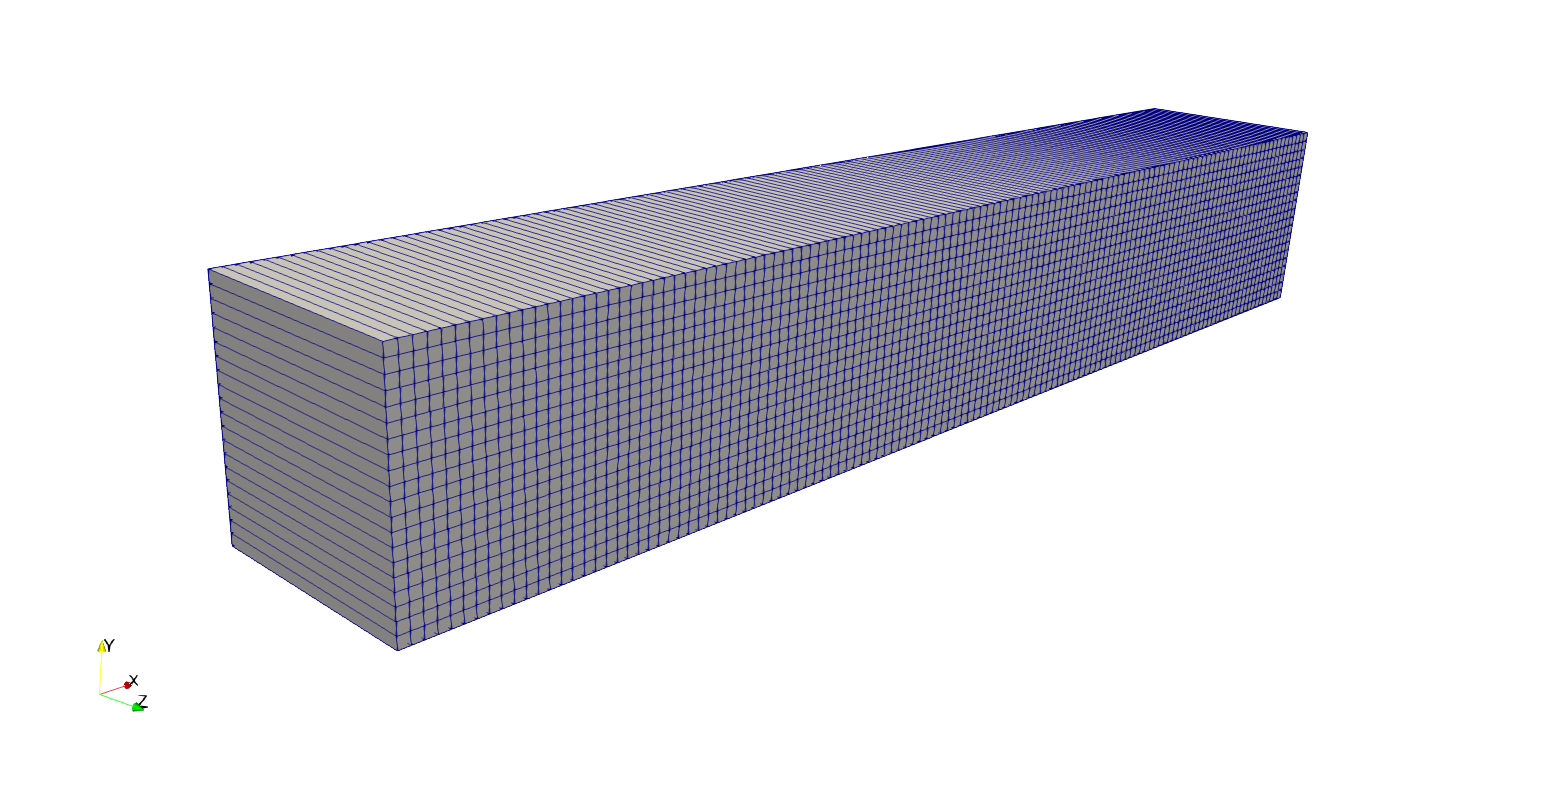
\includegraphics[width=\textwidth]{./figs/mesh/2Dmesh.png}
        \caption{Two-dimensional mesh}
    \end{subfigure}

    \begin{subfigure}[]{\textwidth}
        \centering
        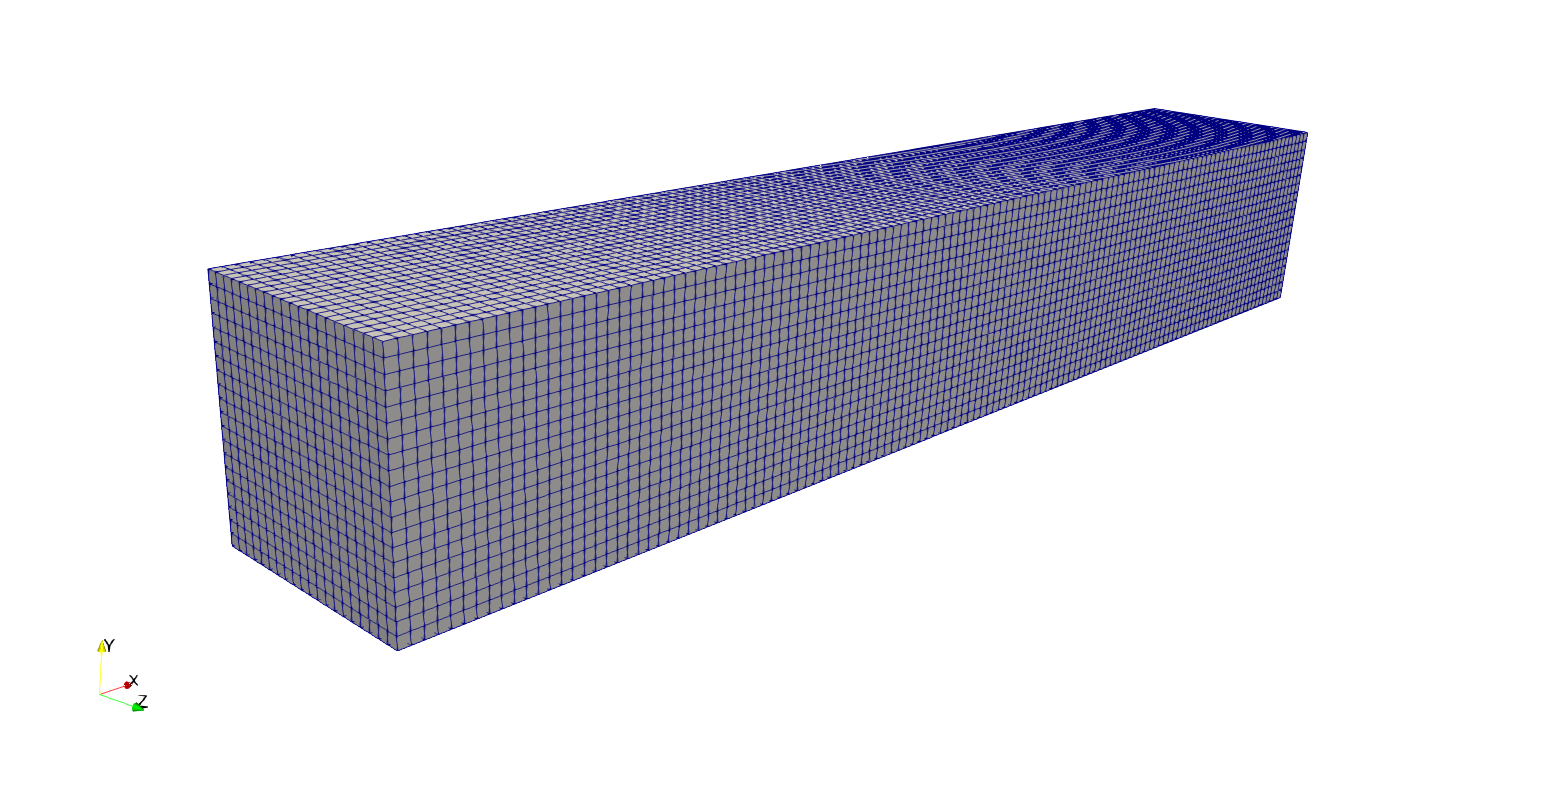
\includegraphics[width=\textwidth]{./figs/mesh/3Dmesh.png}
        \caption{Three-dimensional mesh}
    \end{subfigure}
    \caption{Static meshes used in OpenFOAM for detonation modeling, at an exaggerated unrefined resolution for example purposes}
    \label{fig:meshcompare}
\end{figure}


%%%%%%%%%%%%%%%%%%%%%%%%%%%%%%%%%%%%%%%%%%%%%%%%%%%%%%%%%%%%
%%%%%%%%%%%%%%%%%%%%%%%%%%%%%%%%%%%%%%%%%%%%%%%%%%%%%%%%%%%%
%%%%%%%%%%%%%%%%%%%%%%%%%%%%%%%%%%%%%%%%%%%%%%%%%%%%%%%%%%%%


\section{Detonation Initiation}
\label{sec:ignition}

The initiation of a detonation is seemingly trickier computationally than it is experimentally. There are several methods to do this. Typically, a region of high temperature and pressure gas is instantiated at one end of the tube, such that the fuel and oxidizer ignites within the tube. If the pressure and temperature conditions within this ignition region are high enough, detonation will occur. If they are not, it is possible to instead just ignite the gas and send a decoupled shockwave down the tube in front of the flame. This is not a detonation and undesirable. 

In addition to the thermodynamic conditions that the ignition region is in, the ignition gas itself can be varied. Some researchers have ignited detonation computationally using a block of high temperature and pressure helium \cite{marcantoni}. Towery has used a an ignition block of high temperature and pressure stoichiometric reactants \cite{towery1} as well as a high temperature and pressure gradient \cite{towery2} ranging from higher pressure and temperature near the ignition wall down to the initial condition of the domain. Ignition will be discussed further in \ref{sec:igstudy}.



%%%%%%%%%%%%%%%%%%%%%%%%%%%%%%%%%%%%%%%%%%%%%%%%%%%%%%%%%%%%
%%%%%%%%%%%%%%%%%%%%%%%%%%%%%%%%%%%%%%%%%%%%%%%%%%%%%%%%%%%%
%%%%%%%%%%%%%%%%%%%%%%%%%%%%%%%%%%%%%%%%%%%%%%%%%%%%%%%%%%%%


\section{Initial Attempts}
To begin on the problem of modeling detonations in OpenFOAM, the included tutorials folder as well as the geometric and initial condition setup of located in a related TESLa paper by Towery\cite{towery1} was utilized to begin the work towards an OpenFOAM model of a linear detonation tube/PDE.

Firstly, the detonation of methane fuel and oxygen oxidizer without inert nitrogen filler was explored within a 2D detonation tube with the solver \verb|rhoReactingFoam|. A region of high temperature methane and oxygen on the left hand side was used to initiate the detonation. In the PDE and detonation simulations presented in this paper, stoichiometric fuel and oxidizer was premixed and available thoughout the domain. 
%Solid walls on the left, top, and bottom of the tube were used. The exit was set as a special \verb|waveTransmissive| boundary condition that allows for shockwaves to not reflect at the exit and for gases to expel as well. 
A detonation was successfully created with this, but the accuracy and stability were still untested. In order to check that the boundary conditions being applied were correct, a small detonation cell of high pressure and temperature was set in the bottom left corner of the tube. As the simulation progressed, correct wave reflection was seen on the sides of the tube as well as some wave transmissive behavior from the exit was seen (Figure \ref{fig:cornerdet}). 
\begin{figure}[b]
\centering
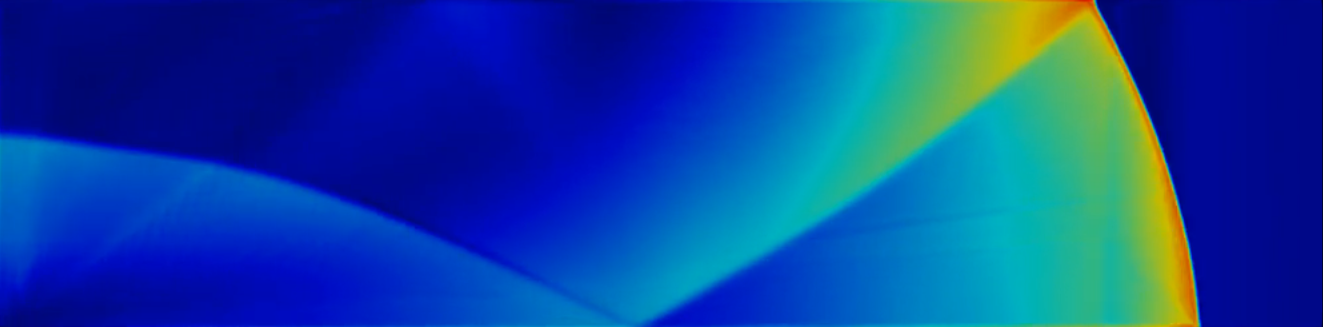
\includegraphics[width=\linewidth]{figs/cornerdet.png}
\caption{Initial methane and oxygen detonation boundary condition test with corner detonation. Velocity magnitude is plotted here without scale to just check the solver and boundary conditions for modeling potential. Detonation was initiated in the lower left corner.}
\label{fig:cornerdet}
\end{figure}%
\noindent It was noticed that the exit boundary condition was expelling gas in a rectangular region long before the detonation wave(s) reached the exit, so some tweaking was done on this \verb|waveTransmissive| boundary condition in order to make it more accurate. The boundary condition option accepts inputs such as ratio of specific heats, expected flow velocity, far-field conditions and distance from exit plane, and names of some variables such as the condition to track at the exit as well as some flux variables. 

The next step with \verb|rhoReactingFoam| was to start progressing towards testable detonation results. To do this, a change from methane to hydrogen for the fuel was selected. This fuel change was done to better match papers such as those being produced by TESLa as well as the general experimental and computational detonation modeling community. The exact geometric detonation tube was taken from Towery\cite{towery1} for comparison as well as the initial detonation size and thermodynamic conditions. Additionally, inert nitrogen was added into the tube to transition from hydrogen-oxygen to hydrogen-air. In accordance with trying to double check whether results made sense with Towery\cite{towery1}, the Arrhenius rate equation was used for reaction rates. An issue that was problematic starting this research was that the documentation for the units within the \verb|reactions| file were conflicting. Much testing was performed at this stage in an attempt to determine the units that OpenFOAM uses for the reactions given in this file, especially regarding the pre-exponential factor. While some ground was gained on this, a shift of focus towards the solver performed in order to determine if \verb|rhoReactingFoam| was appropriate for capturing shocks. 

The Sod shock tube problem was utilized to determine if the OpenFOAM solvers used were capturing shocks accurately. This problem typically consists of placing a region of higher pressure and density fluid in one region and a lower pressure and density fluid in another adjacent region. Typically the regions are rectangular and share a face, both comprising a large cube. When the simulation starts, a shock will form due to the immediate differential in pressure and density from one region to the next. This problem cannot be verified perfectly experimentally, but it can be solved analytically, making this a good method to test numerical CFD solvers for compressible flow accuracy as well as their ability to capture shocks. The results for \verb|rhoReactingFoam| matched published analytical results as well as a \verb|rhoPimpleFoam| case that was matched to the analytical results. Due to this, it was thought that \verb|rhoReactingFoam| would be a good candidate for detonation modeling. 

The next stage consisted of testing different mesh refinement levels, before AMR was utilized. The domain will be expanded on in later chapters, but the domain considered for the initial work is 0.5 meters in length and 0.04 meters square in width. Different static mesh resolutions were tested, such as 5000-1-1, 5000-3-3, 1000-80-1, 1000-3-1, and 10000-2-1. Additionally, some different time steps were tested. At this stage, it was found that there was significant noise and instability in the detonation wave solution, such that consideration of a different solver was advisable. Example results for problems can be seen in Figure \ref{fig:rrf}. 
\begin{figure}[]
\centering
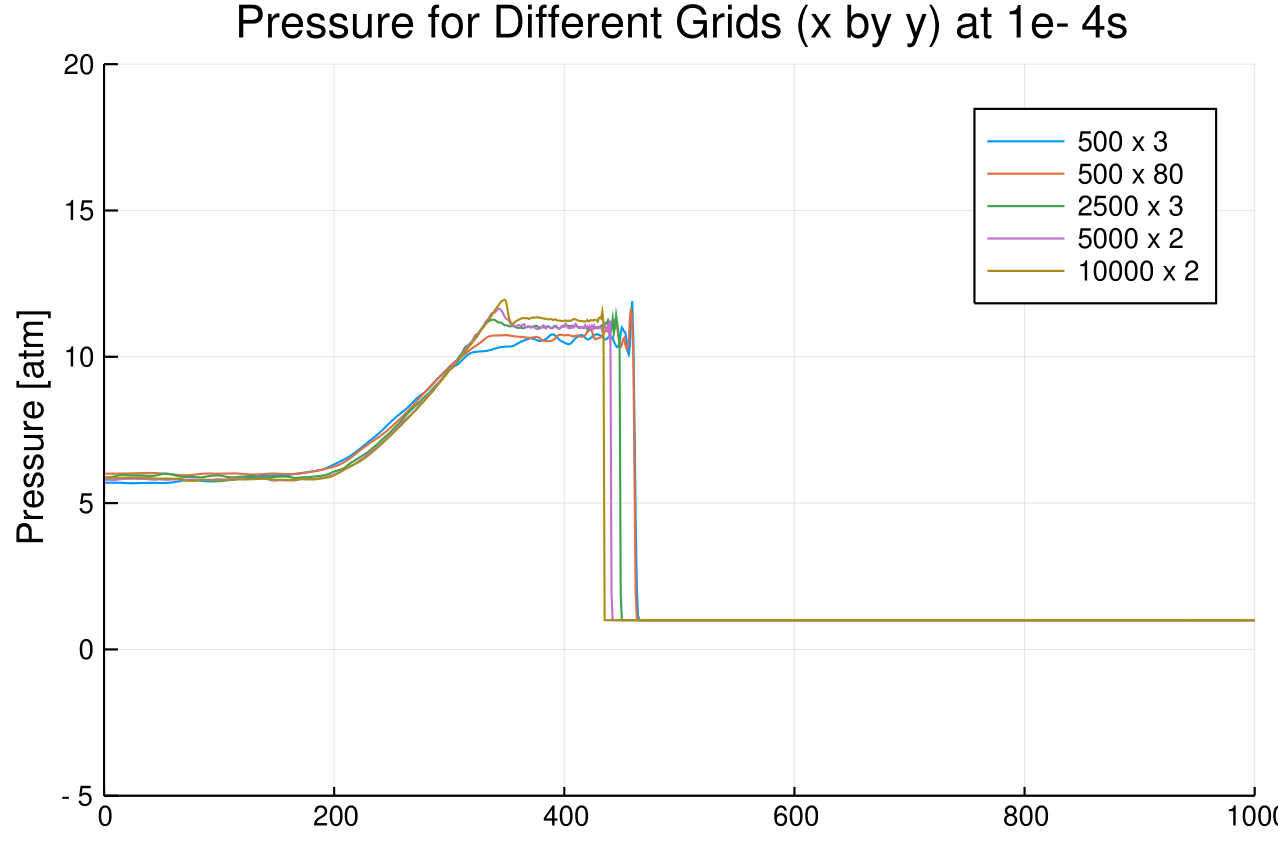
\includegraphics[width=0.85\textwidth]{./figs/rhoReactingFoam.png}
%\caption{Noise and instability in solution and shock capturing problems using \verb|rhoReactingFoam|}
\caption{Noise and instability in solution and shock capturing problems using the \texttt{rhoReactingFoam} solver}
\label{fig:rrf}
\end{figure}%
\noindent We next tried moving towards OpenFOAM solvers utilizing central-upwind schemes of Kurganov and Tadmor, as they should perform better for detonations due to their design around compressible flow. 


%%%%%%%%%%%%%%%%%%%%%%%%%%%%%%%%%%%%%%%%%%%%%%%%%%%%%%%%%%%%
%%%%%%%%%%%%%%%%%%%%%%%%%%%%%%%%%%%%%%%%%%%%%%%%%%%%%%%%%%%%
%%%%%%%%%%%%%%%%%%%%%%%%%%%%%%%%%%%%%%%%%%%%%%%%%%%%%%%%%%%%


\section{Final Solver}

The final solver settled on for this research was \verb|rhoReactingCentralFoam|. This is a solver combined together by Caelan Lapoint from \verb|rhoReactingFoam| and \verb|rhoCentralFoam| and the testing and validation of it is part of this thesis work. First, \verb|rhoReactingCentralFoam| was tested to see if it was accurately capturing shocks like its sister solver, \verb|rhoCentralFoam|. OpenFOAM includes a validated shock tube case utilizing \verb|rhoCentralFoam|, so the results of this were compared to \verb|rhoReactingCentralFoam|'s results in Figure \ref{fig:sod}. 
\begin{figure}[]
\centering
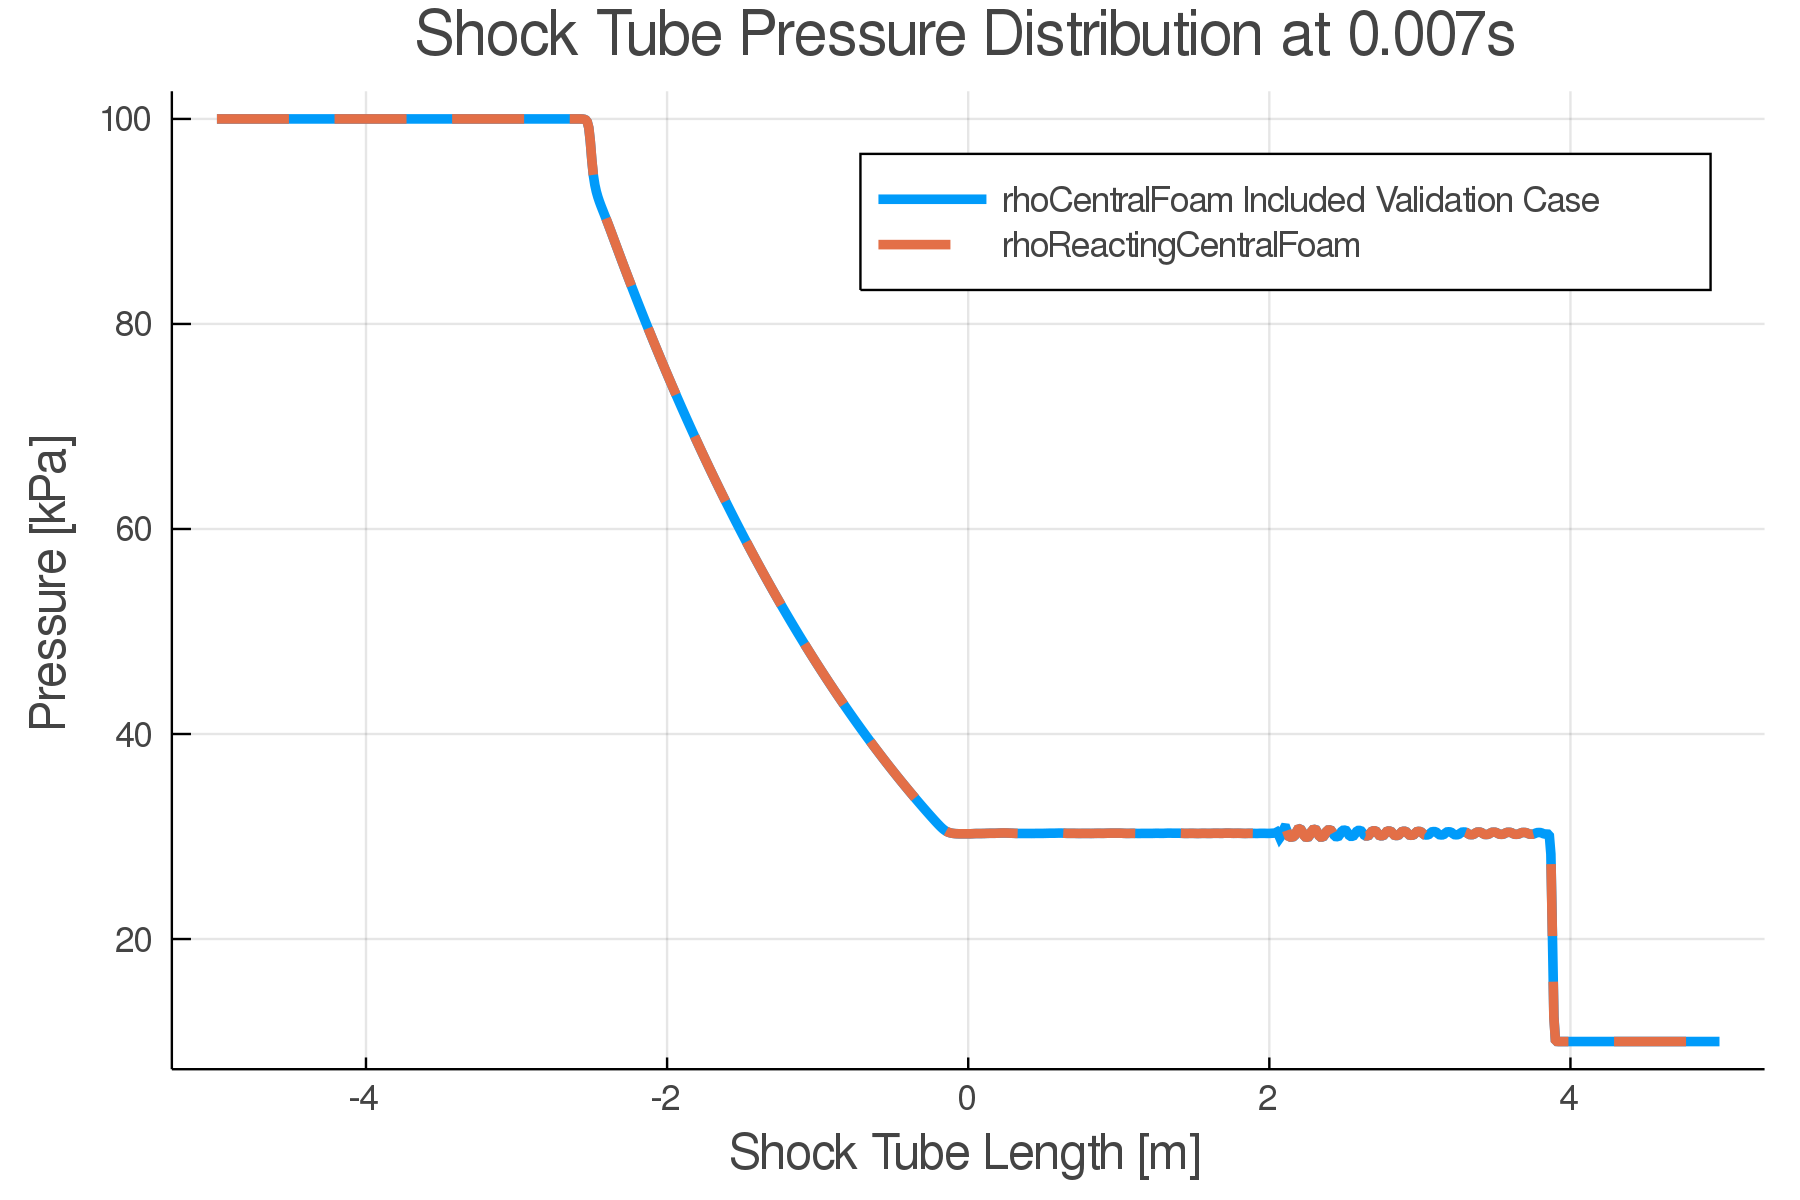
\includegraphics[width=0.85\linewidth]{./figs/shocktube.png} 
\caption{Shock tube validated test case included with OpenFOAM compared to hybrid solver}
\label{fig:sod}
\end{figure}%
\noindent It can be seen that the validation case and \verb|rhoReactingCentralFoam| match precisely, and this was expected. Better numerical stability and less noise was seen in the solutions when moving to 
